Before we move on, we present a simple toy example on the classic two moons dataset, which we augment with a weather-analogue variable. Here, we set $w\in [0,1]$, where being below a given threshold generates the nominal distribution of points in 2D space
\[
    \theta \sim \mt U(0, \pi),\quad \rx \sim\mt N(\cos\theta - 0.5, 0.1), \quad \ry \sim \mt N(\sin \theta - 0.25, 0.1)
\]
and being above the threshold generates the failure distribution from
\[
    \theta \sim \mt U(\pi, 2\pi),\quad \rx \sim\mt N(\cos\theta + 0.5, 0.1), \quad \ry \sim \mt N(\sin \theta + 0.75, 0.1),
\]
in the same way as \cite{dawson2025rare}, where $\mt U$ denotes the uniform distribution. We consider the actual point here to be the latent variable $z$, and add Gaussian noise to it to obtain observations $x$. Then, we attempt to learn an approximation for the posterior $\pld{z\given x,w}$, for each range of $w$, failure and nominal.

\begin{figure}[htb!]
    \centering
    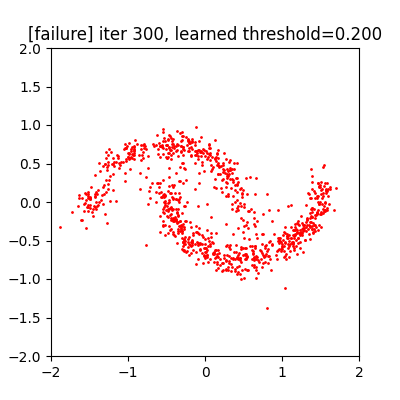
\includegraphics[height=7.5cm]{media/Figure_1A.300.png}
    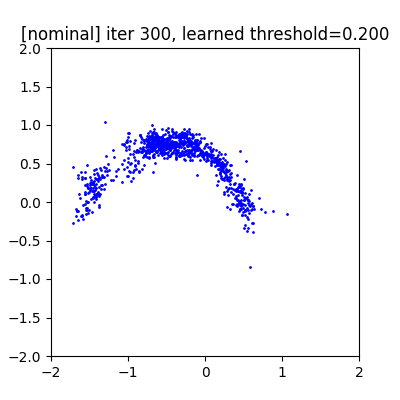
\includegraphics[height=7.5cm]{media/Figure_2A.300.png}
    \caption{Samples from two moons learned posteriors, with incorrectly specified threshold.}
    \label{fig:2moons-bad}
\end{figure}

\begin{figure}[htb!]
    \centering
    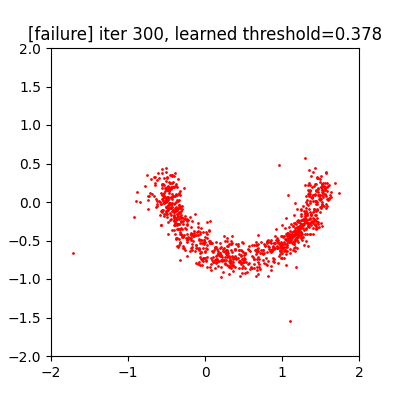
\includegraphics[height=7.5cm]{media/Figure_1.300.png}
    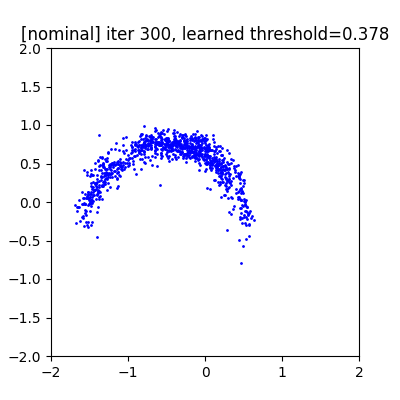
\includegraphics[height=7.5cm]{media/Figure_2.300.png}
    \caption{Samples from two moons learned posteriors, with correct learned threshold.}
    \label{fig:2moons-good}
\end{figure}

\cref{fig:2moons-bad} shows the result when the threshold is incorrectly specified, and \cref{fig:2moons-good} shows the result when the threshold is simultaneously learned. Here, we use a normalizing flows architecture to learn posteriors. As we can see, it is important to ensure that that if we are learning separate posteriors, that they are primarily learned on the data that we are interested in. In the case of the air traffic problem, it is part of the reason why it can be problematic to just classify days into failure or nominal purely based on observed delay or weather, because if our classification is wrong or we do not yet have a clear understanding of how those relate to different regions of the latent space, we may obtain inaccurate or less useful results.